\chapter{Serveur}

\section{Architecture générale}

Le serveur de ce projet est composé de trois principaux modules représentant les différents besoins du projet. Ainsi, il nous faut traiter les données d'entrées fournies par l'utilisateur sous la forme d'un document scanné et possiblement d'une vérité terrain afin de les transformer en données utilisables par les reconnaisseurs. Il nous faut également pouvoir stocker les bases d'apprentissage qui constituent le coeur de notre projet. Enfin, ces bases ne serviraient à rien s'il n'était pas possible d'interfacer notre projet avec le reconnaisseur de l'utilisateur.

Notre projet étant composé de parties bien distinctes, la mise en place de modules indépendants et pouvant être remplacés par l'utilisateur n'a donc pas posé de problèmes. Nous avons donc créé une structure constituée des différents packages correspondant aux fonctionnalités ainsi qu'une interface faisant le lien entre tous. De cette manière, chaque partie est détachée de l'ensemble global et l'interface centrale qu'on appellera \texttt{Controller} fera appel aux méthodes nécessaires des différents packages afin de répondre aux demandes de l'utilisateur. Les packages auront alors une interface à implémenter permettant une utilisation indépendante de l'implémentation.

\begin{mdframed}[frametitle={Architecture des modules avec le connecteur}, innerbottommargin=10]
\begin{center}
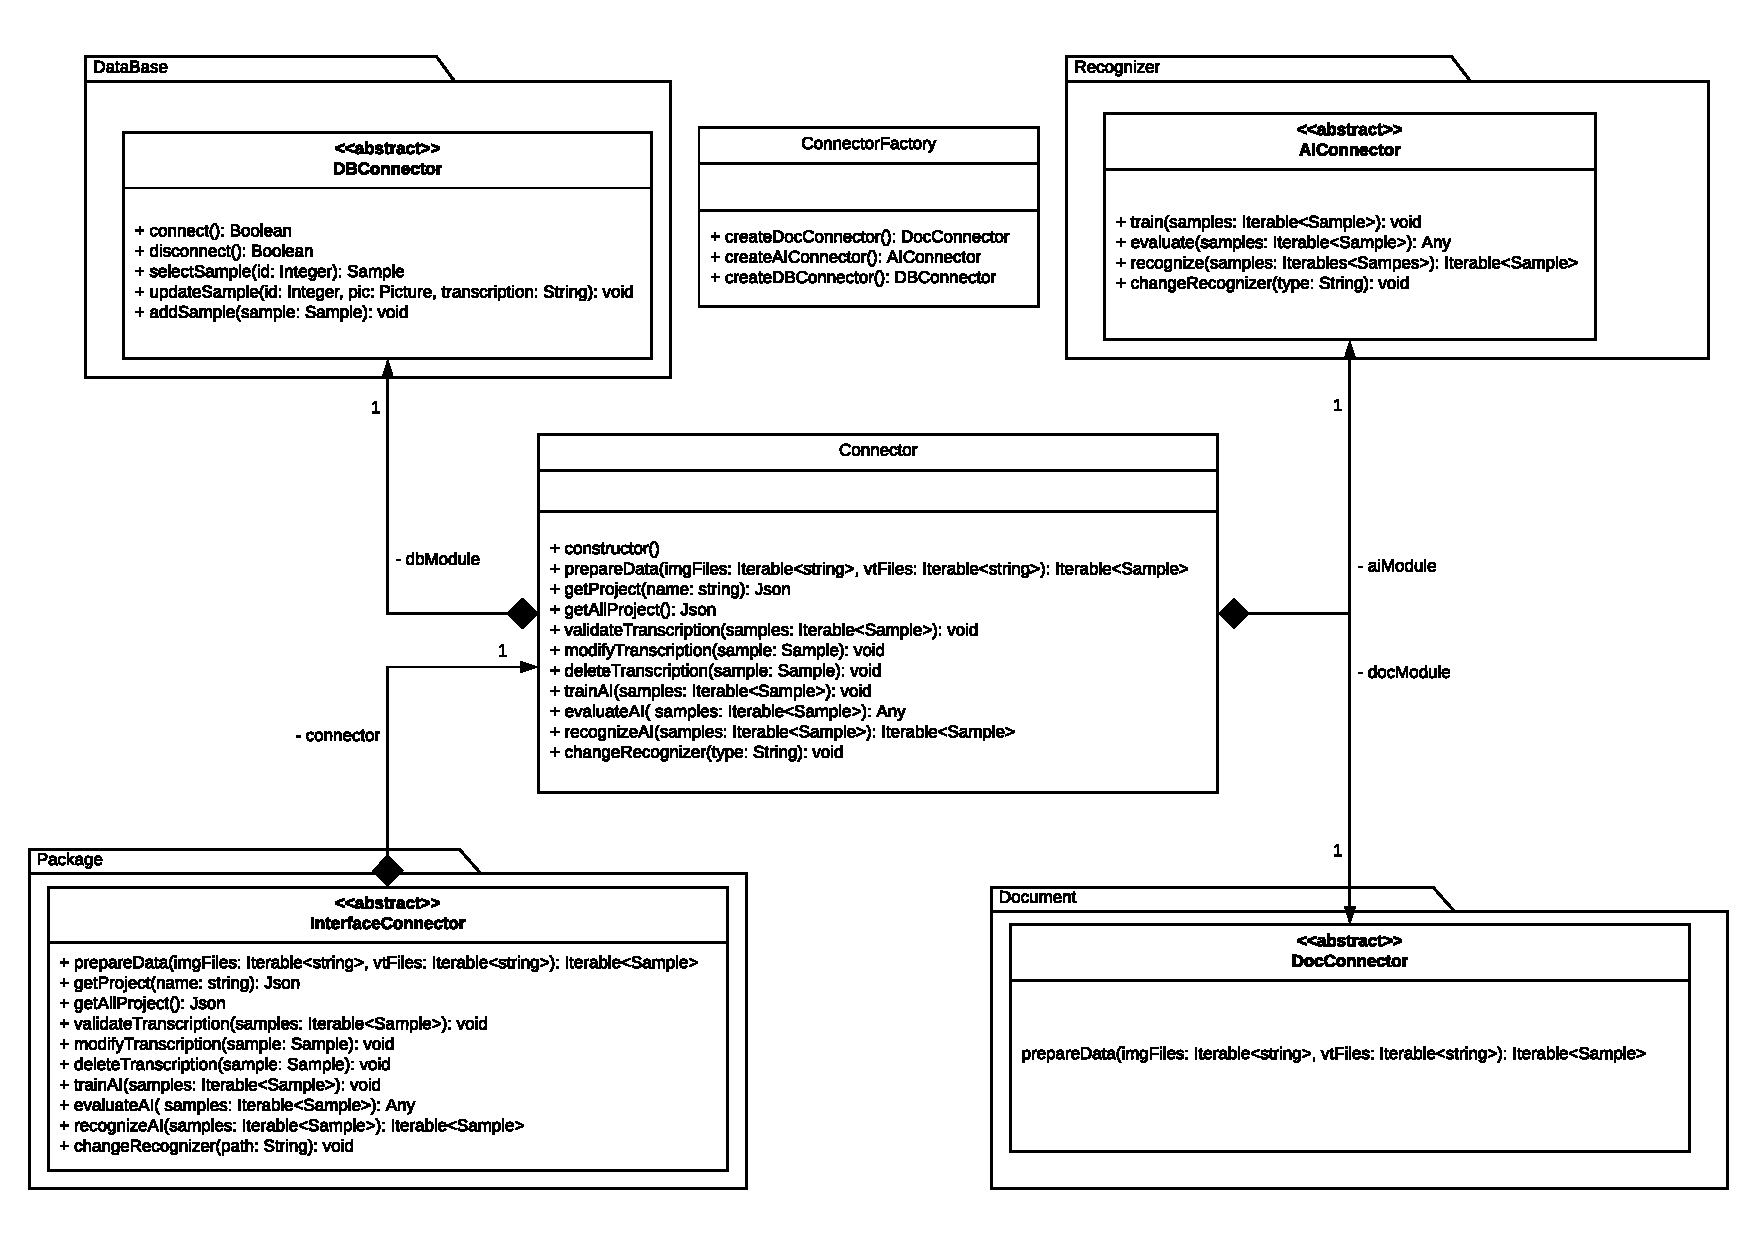
\includegraphics[trim={14cm, 0, 6cm, 0} ,scale=0.3, width=200mm]{assets/UML_connecteur.pdf}
\end{center}
\end{mdframed}

\paragraph{}
Dans notre projet, nous aurons également besoin de représenter les objets avec lesquels nous travaillons. Ainsi, nous avons choisi d'implémenter des classes de données pour représenter les exemples d'apprentissage (\texttt{Example}), les pages des documents utilisés (\texttt{Page}), les-dit documents (\texttt{Document}) et enfin les projets (\texttt{Project}) car on peut imaginer que l'utilisateur puisse vouloir avoir un projet sur des archives paroissiales et un autre sur des textes arabes anciens.


\section{Contrôleur}
\subsection{Architecture}

Le rôle du contrôleur est de mettre en relation les 4 parties du projet : le \textit{frontend}, \textit{i.e.} l'interface homme-machine, la base de données, ainsi que le traitement des données. Pour ce faire, nous avons 4 classes abstraites, un connecteur par \textit{package} du projet, chacun possédant des méthodes générales, qui appellent d'autres méthodes de leurs \textit{packages} respectifs. Cela permet d'avoir un objet \texttt{Controller} central qui manipule tous les éléments du projet avec un code très lisible. Nous fournissons une implémentation de chaque connecteur, pour le bon fonctionnement du projet. Une fabrique est également prévue, permettant de choisir l'implémentation des connecteurs de chaque partie sans avoir à modifier le code du connecteur central. En effet, le contrôleur récupèrera les instances des connecteurs à partir de cette fabrique. Cela permet à l'utilisateur de changer d'instance de connecteur en changeant une ligne de code seulement.

\subsection{Interactions}
\paragraph{}
Le connecteur central reçoit donc, au travers du connecteur en relation avec le frontend les demandes de l'utilisateur et, afin d'exécuter ces demandes, appelle au travers des connecteurs des autres modules, les méthodes nécessaires. Le \texttt{Controller} sert alors d'intermédiaire entre l'utilisateur et les différents modules. Il permet notamment cette structure modulaire en détachant les appels de méthode des classes réelles qui peuvent alors être changées selon le bon vouloir de l'utilisateur.

%-----------------------------------------------------------------------------------------------------------------------
\section{Traitement des données}

Pour ce qui est du traitement des données, il nous faut un \textit{package} pour chacune des deux tâches concernées, à savoir la lecture des fichiers d'entrée ainsi que la découpe d'image.

\subsection{Lecture des fichiers d'entrée : \textit{package} \texttt{input}}

Comme expliqué dans le dernier rapport, nous avons choisi de ne traiter qu'un seul format dans notre logiciel, le format PiFF. Pour pouvoir lire les fichiers d'entrée, on doit construire une représentation des données contenues dans ces derniers sous la forme d'objets. Ceci constituera le \textit{package} \texttt{piff}. Il définit une classe \texttt{PiFF}, qui contient des pages (\texttt{PiFFPage}), qui elles-mêmes contiennent des portions de texte (\texttt{PiFFElement}). Ces classes peuvent être converties au format JSON (bibliothèque \href{https://mvnrepository.com/artifact/org.json/json}{org.json}), ce qui permet d'exporter les objets vers un fichier PiFF.

\paragraph{}
L'utilisateur doit toutefois pouvoir utiliser d'autres formats. Pour cette raison, nous avons un \textit{package} \texttt{converters} contenant une interface, \texttt{PiFFConverter}, qui permet de convertir un fichier quelconque en objet \texttt{PiFF}. Nous en fournissons une implémentation, l'objet \texttt{GEDIToPiFFConverter}, qui permet au logiciel de lire le format GEDI, utilisé notamment par la base de données Maurdor, présentée dans les précédents rapports, et à laquelle nous avons accès pour nos tests. L'utilisateur peut rajouter autant d'implémentations qu'il le souhaite.

\paragraph{}
En plus de ces deux \textit{packages}, nous proposons un objet \texttt{PiFFReader} (singleton), qui permettra d'ouvrir un fichier, et d'utiliser les concepts présentés ci-dessus. Plus précisément, il permettra de lister des implémentations de \texttt{PiFFConverter}, et de les appeler une par une sur le fichier d'entrée pour réussir à le lire.

\subsection{Découpe des images : \textit{package} \texttt{processing}}

Pour la découpe d'image, il nous faut une classe \texttt{ImageProcessing}, qui appelle les méthodes de la bibliothèque OpenCV, que nous avons choisie précédemment. Après la découpe, les imagettes sont associées au texte pour former des exemples, que nous avons modélisés par une classe \texttt{Example}. 

\paragraph{}
La phase de découpe étant automatique, il nous faut faire appel à un détecteur de lignes. C'est la fonction du \textit{package} \texttt{linedetection}. Nous y plaçons une interface \texttt{LineDetector}, qui permet de trouver les lignes de texte dans un objet PiFF. Le détecteur de lignes utilisé pour le projet est fourni par l'encadrant, et fonctionne sous Linux. Les membres du groupe peuvent pourtant travailler sous Windows ou macOS. Pour faciliter le développement du logiciel, nous avons donc choisi de fournir une implémentation, la classe \texttt{BlurLineDetector} (nom dû à la méthode de détection), basée sur des connexions réseau, afin de pouvoir faire fonctionner le serveur sous n'importe quel système d'exploitation, avec un petit module serveur sous Linux qui appelle simplement l'exécutable. Ce petit module ne fait pas partie du cahier des charges mais sera développé pour les tests. L'utilisateur, ici aussi, pourra rajouter ses propres méthodes de détection de lignes s'il le souhaite.

%-----------------------------------------------------------------------------------------------------------------------
\section{Base de données}

Le Système de Gestion de Bases de Données (SGBD) choisi est SQLite. Le contenu des tables ainsi que l'UML de ce module du projet ont déjà été imaginés par les membres de l'équipe qui sont en mobilité ce semestre. La bibliothèque Java SQLite, une implémentation de l'API JDBC (Java DataBase Connectivity), nous servira à appeler des commandes SQL directement depuis notre programme. Elle nous est également fournie. Il ne nous reste donc plus qu'à implémenter ce module ainsi qu'à l'intégrer dans le projet.

Pour ce faire, on utilise une classe (...)

%-----------------------------------------------------------------------------------------------------------------------
\section{Interface avec le reconnaisseur}

Cette partie du projet a pour objectif de lier la base d'apprentissage de notre logiciel avec le reconnaisseur choisi par l'utilisateur. Ainsi, cette partie étant très liée à l'utilisateur, il faut lui permettre de pouvoir facilement attacher le reconnaisseur de son choix au logiciel. C'est avec cette contrainte en tête que nous avons conçu l'architecture de cette partie.

\begin{mdframed}[frametitle={Architecture de l'interface avec le reconnaisseur}, innerbottommargin=10]
\begin{center}
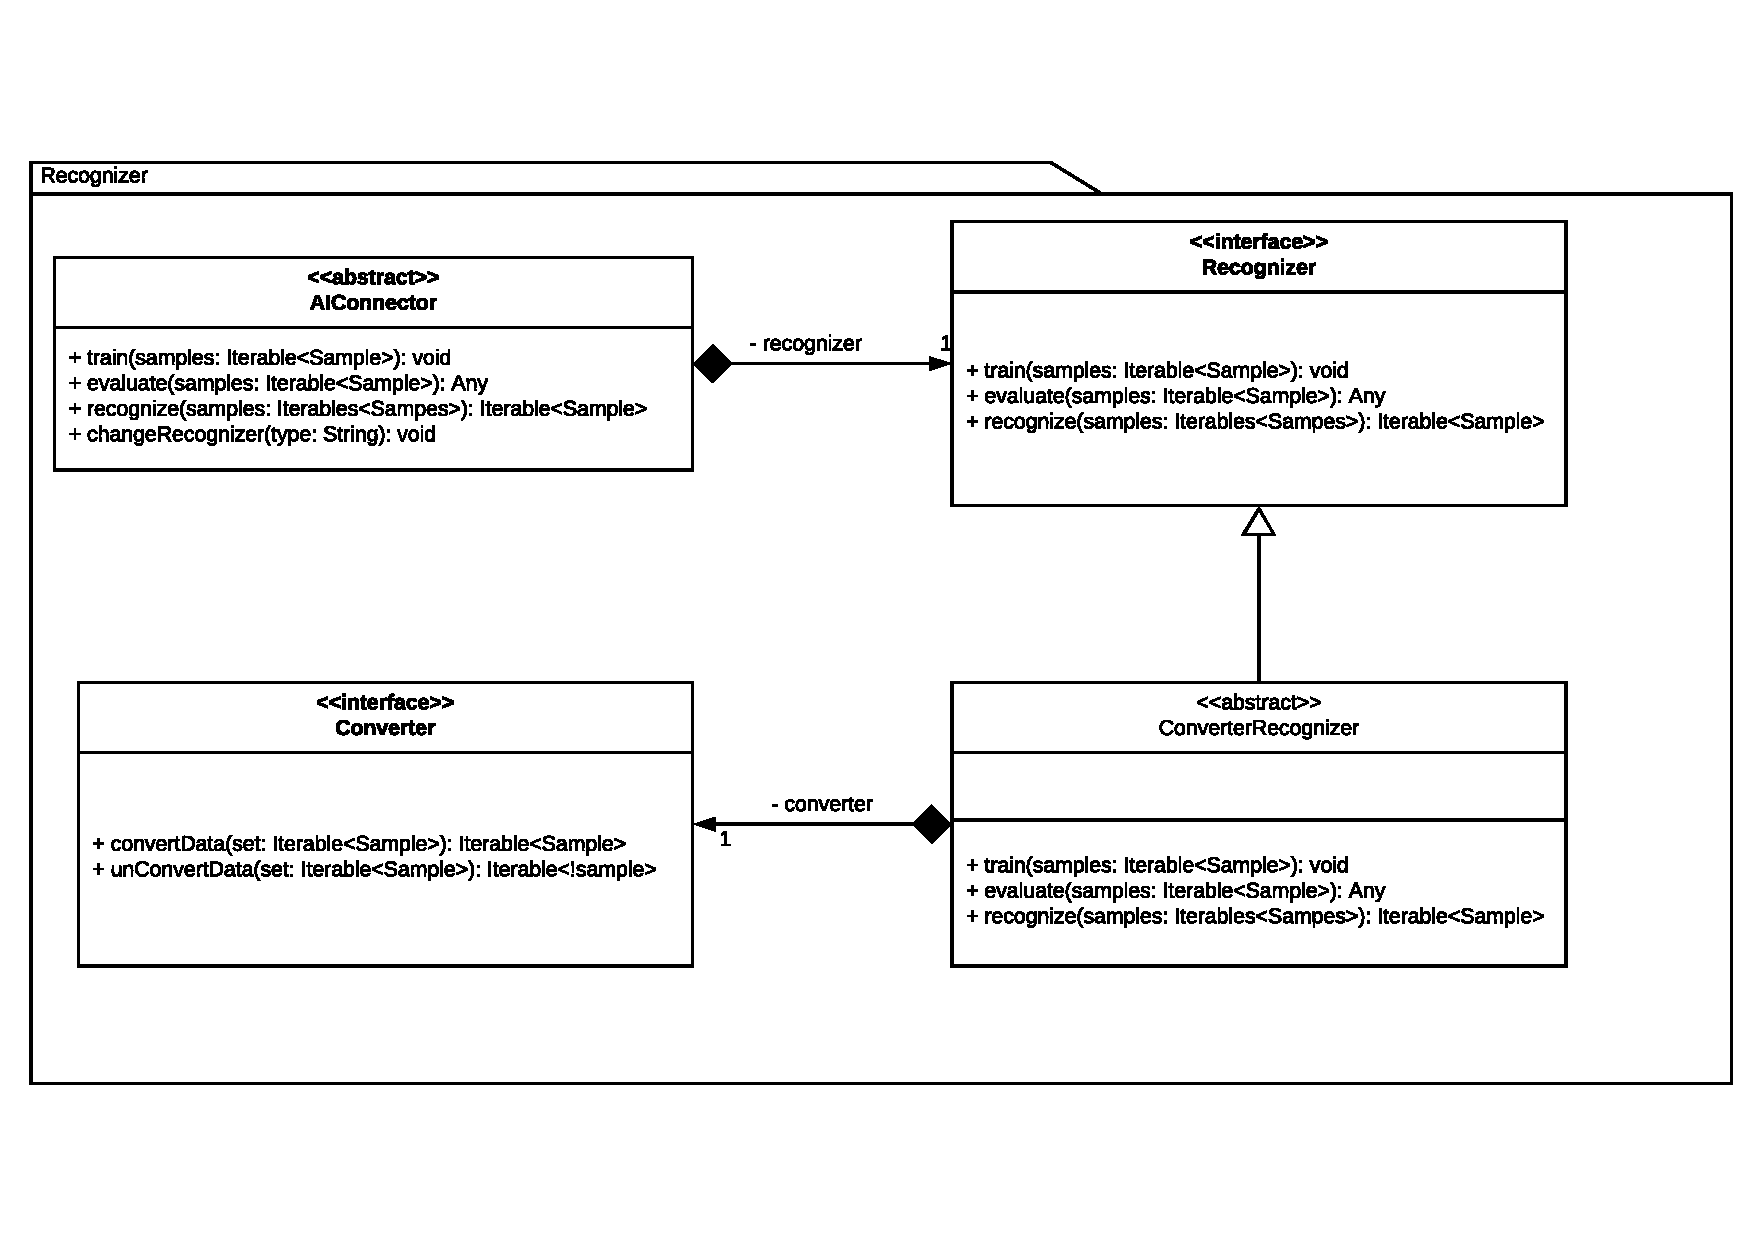
\includegraphics[trim={0, 2cm, 0 , 7cm}, scale=0.55, height=100mm]{assets/UML_Recognizer.pdf}
\end{center}
\end{mdframed}

\paragraph{Architecture}

Cette partie du projet contient comme toutes les autres un connecteur qui la lie au \texttt{Connector} principal. Ce connecteur possède un \texttt{Recognizer} afin de pouvoir effectuer les opérations classiques d'entrainement, d'évaluation de celui-ci ainsi que lui demander d'effectuer une transcription. Il permet également de changer de reconnaisseur quand l'utilisateur souhaite utiliser un autre type de reconnaisseur.
\newline{}
Le reconnaiseur est représenté par une interface \texttt{Recognizer} qui permet trois actions possibles: entrainer le reconnaisseur à partir d'un ensemble d'apprentissage, évaluer ce même reconnaisseur sur un ensemble de validation, et enfin, lui demander de transcrire un ensemble non étiqueté.
Cette interface permet notamment à l'utilisateur, de connecter son propre reconnaisseur, et même s'il le souhaite, d'en créer un au sein de l'application. Elle est également la seule qu'il est obligé d'implémenter pour faire fonctionner l'ensemble. Cependant, il faut dans certains cas convertir les données dans la base de donnée en données compréhensibles par le reconnaisseur. Ainsi, deux autres interfaces sont nécessaires: une interface \texttt{Converter} permettant la convertion des données entrantes et sortantes du reconnaisseur ainsi qu'une classe abstraite \texttt{ConverterRecognizer} héritant de \texttt{Recognizer} et possédant un convertisseur adapté au reconnaisseur utilisé. En effet, le reconnaisseur peut avoir besoin d'un formatage des images en entrée, mais également de la transcription associée. Par exemple, nous implémenterons la structure décrite précédemment pour un reconnaisseur particulier: \href{https://github.com/jpuigcerver/Laia}{Laia}. Ce reconnaisseur demande de transformer les images afin qu'elles aient la même hauteur en pixel et que la transcription soit traduite dans les symboles qu'il peut reconnaitre et organisée d'un certaine façon. Par exemple, il faut remplacer les  ' ' par '<space>' et que l'identifiant de l'image correspondante à la transcription soit indiqué avant celle-ci dans un fichier. Le convertisseur va donc se charger de mettre en forme les données et de créer ce qui est nécessaire.
\newline{}
Dans la première version délivrée le 27 Février, la possibilitée d'entrainer le reconnaisseur doit être implémentée ainsi que celle de changer de reconnaisseur. Dans un second temps, il sera possible de faire transcrire les imagettes par le reconnaisseur et de faire l'évaluation de celui-ci. Les données remontées lors de l'évaluation sont laissées libres à l'utilisateur puis que la fonction rend un objet non défini à l'avance qui sera sous la forme d'un \textit{JSON} et qui contiendra les informations choisies par l'utilisateur dans son implémentation. Il pourra alors obtenir le nombre et la fréquence des erreurs, sur quelles lettres celles-ci surviennent, et ainsi de suite.

\paragraph{Interactions}
L'interface avec le reconnaisseur sert de passerelle entre le noyau du projet qui est le connecteur central et le reconnaisseur que l'utilisateur souhaite utiliser. Ainsi, elle reçoit au travers de son propre connecteur (\texttt{AIConnector}) les ensembles d'\texttt{Example} à utiliser pour ses différents usages. L'implémentation de l'interface \texttt{Recognizer} se charge ensuite, de transmettre au reconnaisseur soit sous forme de jar, soit installé sur la machine de l'utilisateur les données d'exemple dans le format approprié. Lorsqu'il reçoit les réponses du reconnaisseur, il les convertit de nouveau en Example qui pourront être manipulé par le logiciel en interne.

%-----------------------------------------------------------------------------------------------------------------------
